\documentclass[conference]{IEEEtran}
\IEEEoverridecommandlockouts
% The preceding line is only needed to identify funding in the first footnote. If that is unneeded, please comment it out.
\usepackage{cite}
\usepackage{amsmath,amssymb,amsfonts}
\usepackage{algorithmic}
\usepackage{graphicx}
\usepackage{textcomp}
\usepackage{xcolor}
\def\BibTeX{{\rm B\kern-.05em{\sc i\kern-.025em b}\kern-.08em
    T\kern-.1667em\lower.7ex\hbox{E}\kern-.125emX}}
\begin{document}

\title{5G UE Classification Framework Using Network Analytics\\
{\footnotesize \textsuperscript{}}
}

\author{
\IEEEauthorblockN{Hemendu Roy}
\IEEEauthorblockA{\textit{Arizona State University} \\
Tempe, USA \\
hroy6@asu.edu}
\and
\IEEEauthorblockN{Nikhil Anantharaman}
\IEEEauthorblockA{\textit{Arizona State University} \\
Tempe, USA \\
nananth6@asu.edu}
\and
\IEEEauthorblockN{Ravindra Aditya Singh}
\IEEEauthorblockA{\textit{Arizona State University} \\
Tempe, USA \\
rsing122@asu.edu}
\and

\IEEEauthorblockN{Thejas Naik}
\IEEEauthorblockA{\textit{Arizona State University} \\
Tempe, USA \\
tanaik@asu.edu}
}

\maketitle

\begin{abstract}
Everyday, the number of mobile devices such as smartphones and wearables grows exponentially. With such rapid growth, comes the demand for a new generation of mobile communication.
Thus, the need for a highly scalable and easily deployable network technology, 5G was born. To meet the diverse requirements of a 5G network, the concept of Network Slicing was introduced.
5G network slicing is a network architecture that enables the multiplexing of virtualized and independent logical networks on the same physical network infrastructure. However, though the concept of 5G Network Slicing has been theorized and even to some extent, tested, User Equipment (UE) Classification has not been given the same attention. In this paper, we propose a three-step architecture to classify UEs in a 5G network and subsequently determine its appropriate Network Slice.
\end{abstract}

\begin{IEEEkeywords}
5G, Network Slicing, User Equipment Classification, Distributed Systems
\end{IEEEkeywords}

\section{Introduction}
In a 4G network, UEs are not segregated based on their functional requirements. Hence, all UEs connect to a singular network and are not prioritised in any fashion. However in 5G Networks, UEs are expected to connect to a particular Network Slice that is designed to serve their specific set of requirements. For example, a UE belogning to an autonomous vehicle system will connect to an eV2X network slice and a UE belonging to an IoT network may connect to an mMTC network slice. In this way, a high degree of QoS i.e. Quality of Service is guaranteed to all connected clients. It is therefore, of prime importance that a framework be developed that correctly classifies connected UEs into their respective usage classes. Such a framework must also account for changes in usage patterns of UEs and  must be able to dynamically re-classify UEs. Additionally, as an added QoS feature, a client may simply be given a nertwork slice recommendation along with the freedom to choose any network slice.

\section{System Architecture}
When a UE is on-boarded onto a 5G Network, they will be connected to a generic, smaller network for a short ‘trial period’ of one week. During this period, the user’s network usage patterns will be analysed using an intelligent classification framework inspired by \cite{b2} as described below. Once a UE has been successfully classified, it can be assigned to a Network Slice Instance catered to its specific requirements.
\begin{figure*}[htbp]
\centerline{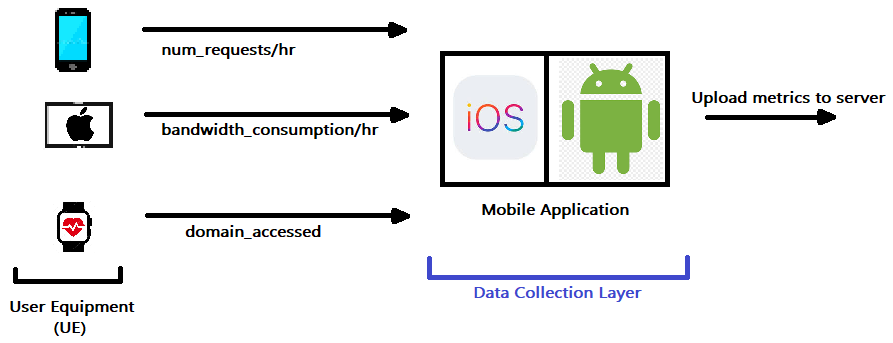
\includegraphics[scale=0.7]{fig1.png}}
\caption{Client Side (a) Data Collection Layer}
\label{dclayer}
\end{figure*}
\begin{figure*}[htbp]
\centerline{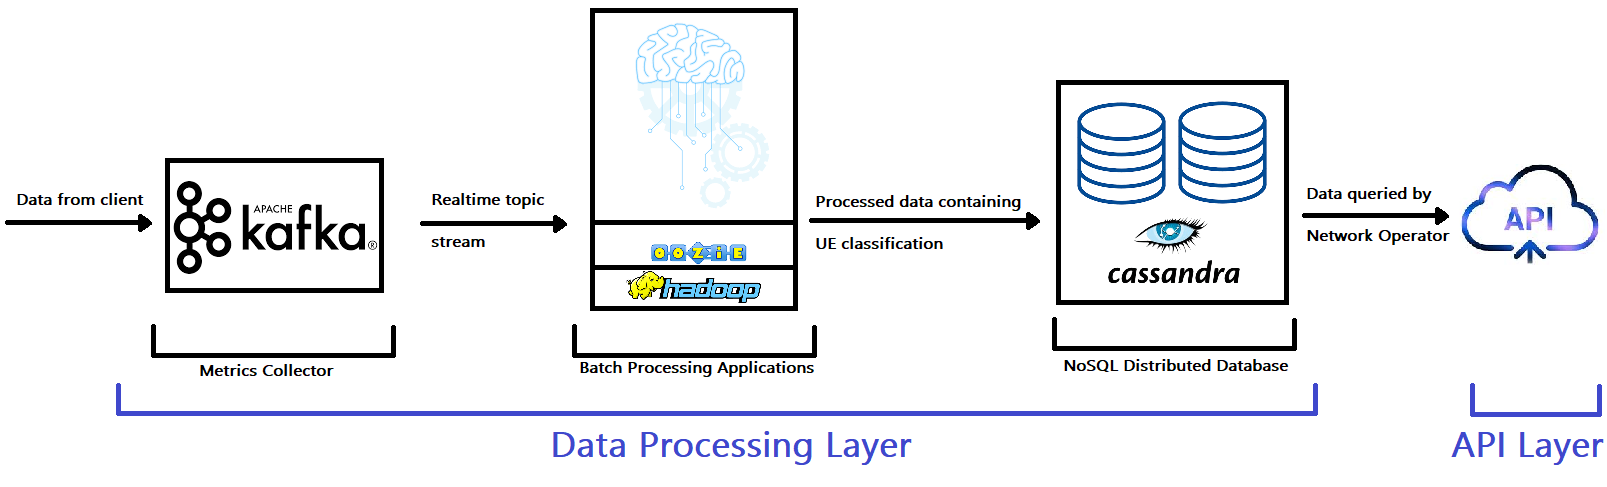
\includegraphics[scale=0.4]{fig2.png}}
\caption{Network Operator Side (a) Data Processing Layer and (b) API Layer}
\label{prlayer}
\end{figure*}
\\
The implementation for this system consists of a three-layer architecture:
\\
As illustrated in Fig ~\ref{dclayer}, the Client Side is comprised of
\begin{enumerate}
\item Data Collection Layer (Android Application)
\end{enumerate}
As illustrated in Fig ~\ref{prlayer}, the Network Operator Side is comprised of
\begin{enumerate}
\setcounter{enumi}{1}
\item Data Processing Layer (Cloud Infrastructure)
\item API Layer
\end{enumerate}

\subsection{Data Collection Layer}\label{AA}
An Android Application will be designed and developed to run on mobile devices such as cell phones, tablets and wearables. The application will collect 5G Radio network related metrics such as,
\begin{enumerate}
\item Bandwidth Consumption per hour
\item Domains Accessed
\item Number of requests made per hour
\end{enumerate}

These metrics will then be sent to the ISP over the network for further processing.

\subsection{Data Processing Layer}
These metrics will be streamed in real time using an event streaming platform such as Apache Kafka. This stream of data will then be periodically consumed by scheduled applications running on an Apache Hadoop Cluster facilitated by AWS EC2 instances that employ a Machine Learning model to classify these users and store the results in a highly scalable Apache Cassandra database.

\subsection{API Layer}
Once users have been classified according to their network requirements, a REST API is used to relay this information to a Network Operator such as AT\&T, Verizon, T-Mobile etc. Now, the Network Operator can assign the user to an appropriate Network Slice Instance.
\\
For example,
\begin{enumerate}
\item In the case of high bandwidth consumption which can be the case if the UE often accesses video streaming platforms, the UE will be connected to an \textbf{Extreme (or enhanced) Mobile Broadband (eMBB)} Network Slice Instance
\item If the UE makes a large number of requests to the Network Operator but exhibits relatively lower bandwidth consumption trends, it can be deduced that it is one of various kinds of IoT devices such as Smart Watches. In this case, the UE will be connected to a \textbf{Massive Machine-Type Communications (mMTC)} Network Slice Instance.
\item In the case it is detected that the UE is making bursts of location related queries, it can be deduced that the device in question may be the processing unit of an autonomous vehicle, for example, an iPad in a Tesla car. The device must then be connected to an Ultra-reliable \textbf{Low-Latency Communications (urLLC)} Network Slice Instance.
\end{enumerate}

\section{UE Classifier Model}

As briefly discussed in the previous section, a Machine Learning model will be used to classify UEs into a set of usage classes which can then be used by a 5G Network Provider appropriately assign Network Slices to UEs. A proposed implementation of such a classification model is described in  Fig ~\ref{uemodel}.

\subsection{Input Dataset}
Once the UE network metrics are received by the system, they will be formatted into 2-D matrices. For example, a set of pairs containing a domain accessed and its frequency. Essentially, this is a tabular representation of the Word Cloud in Fig ~\ref{wordcloud}. Similarly, a matrix representation of ports used can be another input. Additionally, metrics such as bandwidth usage and requests per hour are also stored in 1-D arrays and passed to the classifier.

\subsection{Stage-0 Classifier}
We use a Naive Bayes Multinomial classifier to process each of the matrices and output for each, a tentative class and a corresponding confidence level. Some quantitative metrics such as average bandwidth usage and average number of requests per hour are also computed. The results from the Stage-0 classifier are then fed into a Stage-1 classifier.

\begin{figure*}[ht]
\centerline{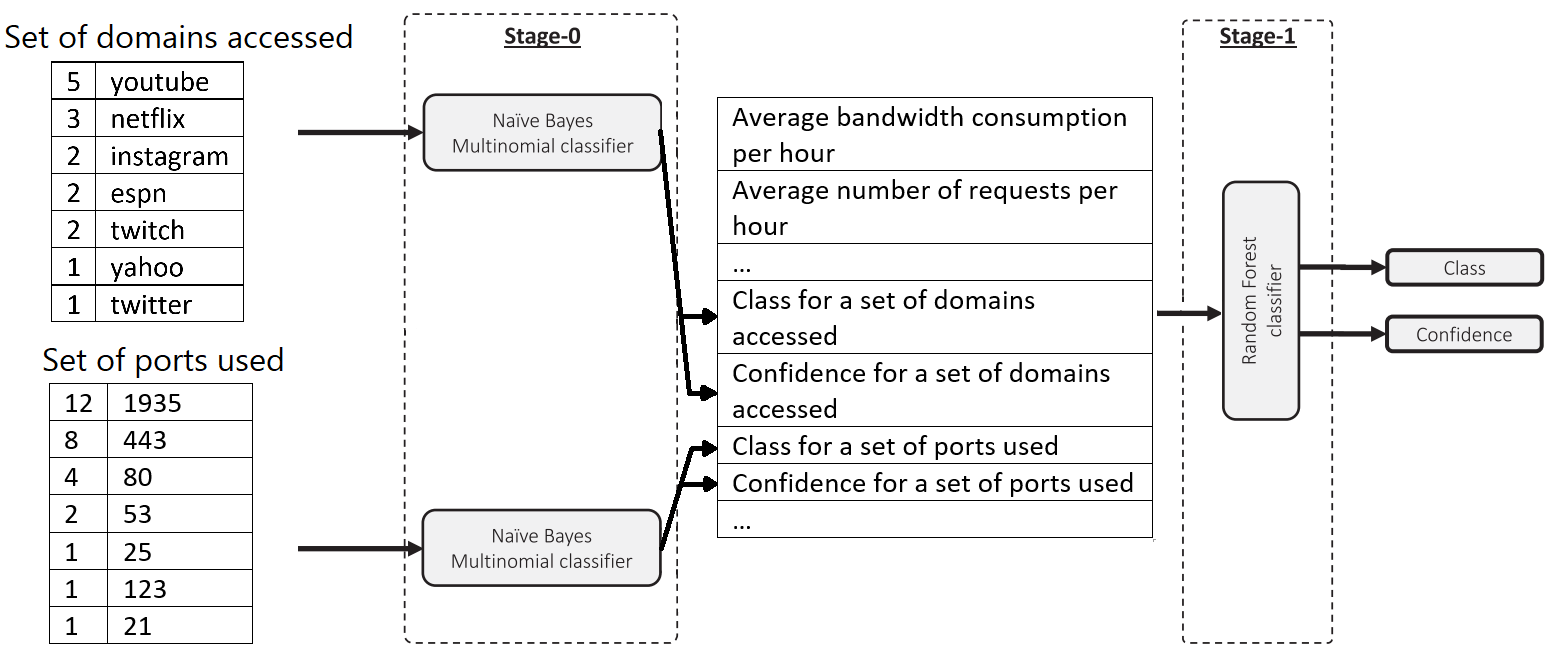
\includegraphics[scale=0.4]{fig5.png}}
\caption{Architecture of the multi-stage UE classifier system}
\label{uemodel}
\end{figure*}

\subsection{Stage-1 Classifier}

This stage uses a Random Forest classifier on the nominal values received from Stage-0. As detailed in \cite{b4}, a key advantage of using a Random Forest is its high tolerance to over-fitting as compared to other decision tree classifiers.


\section{Enhancements}
\subsection{Dynamic Re-classification}
\begin{figure*}[htbp]
\centerline{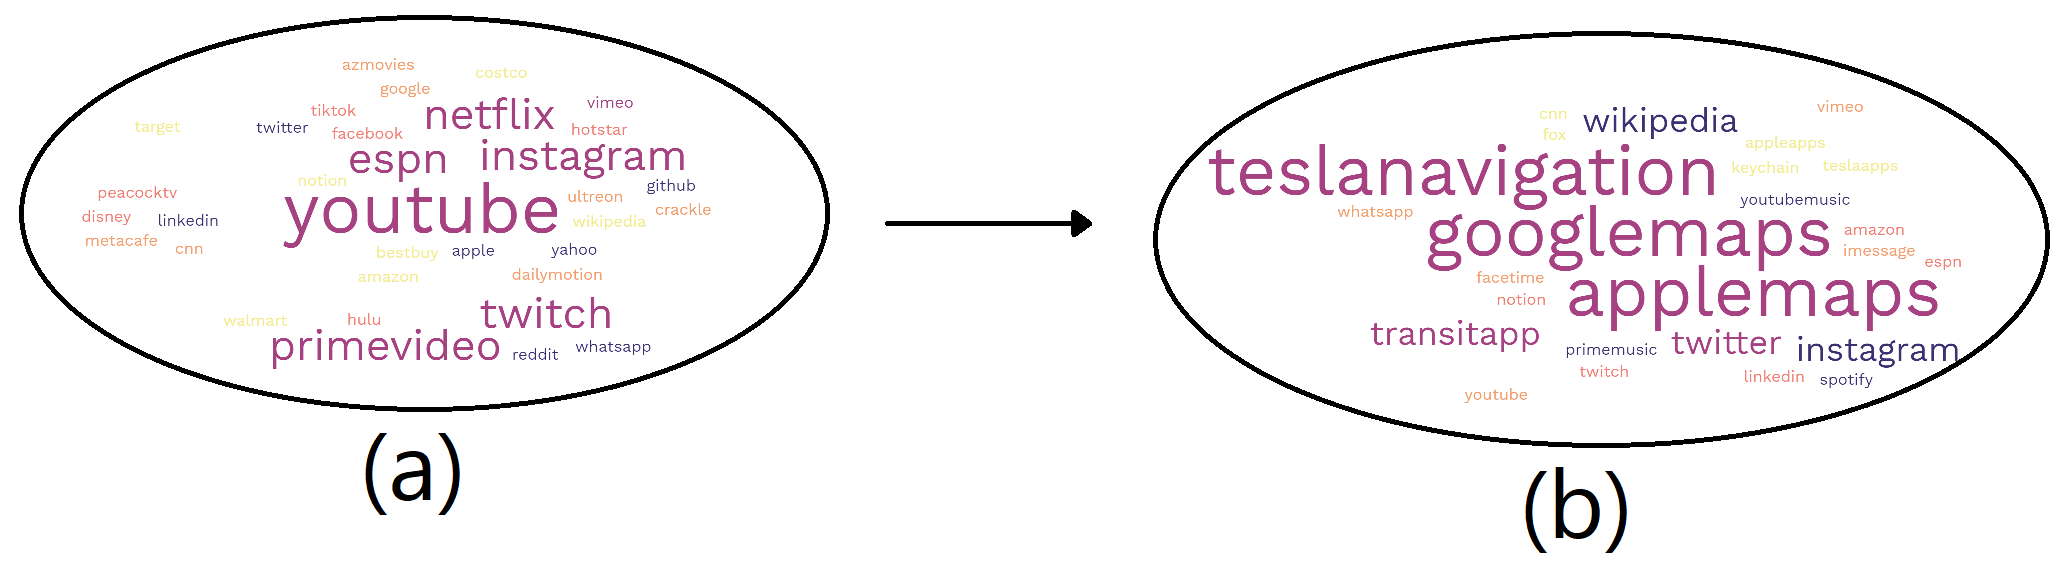
\includegraphics[scale=0.3]{fig3.png}}
\caption{The set of frequently accessed domains by an iPad (a) as part of an eMBB slice and (b) as part of a urLLC slice}
\label{wordcloud}
\end{figure*}
Although rare, it may be possible that a UE that has already been classified into a certain category begins exhibiting vastly different usage patterns from what is expected. For example, an iPad belonging to a daily user would likely belong to an eMBB network slice meant for high video consumption. If however, it was repurposed to be used in a Tesla vehicle, which also uses iPads for their interior controls, the UE would need to be re-classified. If the set of domains accessed by the device were the primary metric considered for these classifications, an analysis of these domains would be the key factor in re-classifying the device.  Fig ~\ref{wordcloud} shows an example of a stark change in the set of domains accessed by the UE due to a change in its functional requirements. It is likely that now, urLLC would be the appropriate network slice for this device as extremely low latency would be of paramount importance to ensure driver safety in a hazardous traffic environment.

Another example in  Fig ~\ref{bwgraph} shows the variation in average bandwidth consumption of a device. In such a case, the variation is so drastic that it reaches levels comparable to those of devices connected to an eMBB network slice. In such a scenario, the UE in question must be moved from its configured network slice to an eMBB network slice. One of the challenges in advanced 5G Network Slicing principles is to facilitate devices that have overlapping requirements. To address such corner cases, multi-layered network slicing is proposed where a set of devices can be effectively connected to more than one network slice and make use of their varying benefits. 
A corresponding change must then be implemented in the UE classification model to allow the assignment of multiple network slices to certain UEs. In order to optimize resource usage, re-classification applications may run at a lower frequency as compared to primary classification jobs. 
\begin{figure}[ht]
\centerline{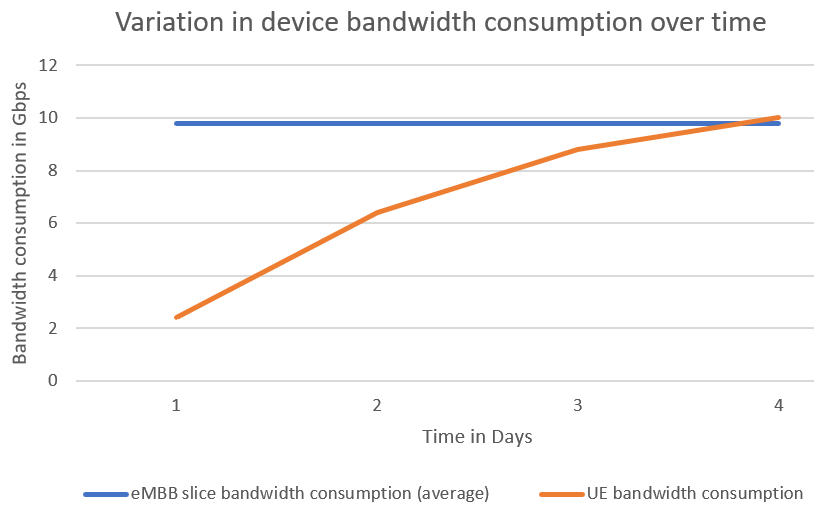
\includegraphics[scale=0.43]{fig4.png}}
\caption{An example of metric variation over time requiring continuous monitoring for re-classification}
\label{bwgraph}
\end{figure}
Say, if the primary jobs are scheduled to run once every 24 hours, the re-classification jobs can be assigned a lower priority and must run not more than once in 72 hours.

\subsection{User-requested re-classification}
In some scenarios, where the user has a certain level of technical expertise, they may explicitly request to join a network slice different from that predicted by the proposed UE Classification framework. For example, a group of individuals involved in drone research may like to repurpose their IoT devices as sensors that require realtime data with minimal latency. In such a scenario, the devices would have to be re-classified from a mMTC network slice to a urLLC slice. However in such a scenario, dynamic reclassification would not be sufficient as it may take several days for a change in metrics to exceed pre-defined baseline thresholds and trigger an automatic re-classification request. Therefore, the user must be given an option to explicitly request an immediate reclassification. A provision may be made in the mobile application to allow a user to submit such a request that is then subject to approval by the network operator. Consequently, the API Layer must also be modified accordingly, to accept and handle such re-classification requests.

\section{Challenges}
\subsection{Lack of datasets for modelling}
Since Standalone 5G networks have not been implemented in a commercial setting yet, datasets that are accurate or even large enough to successfully construct a UE classification model are currently not available. While there are smaller datasets available, these are based on simulated UE traffic and not real data. Therefore, these cannot be considered conclusive. It is likely to take several years of research and work in fields such as Software Defined Networking (SDN) and Network Slicing before a fully functional, large-scale 5G Mobile Network is constructed. Only once such a network is realised, can the feasibility of the proposed UE classification framework be properly assessed.

\subsection{Steep 5G Network Slicing Testbed reqiurements}
In order to successfully design and implement the proposed 5G UE Classification framework, a 5G Network Slicing testbed along with RAN virtualisation including a gNodeB (3GPP-compliant implementation of the 5G-NR base station) and finally, UE traffic simulation is required. \cite{b1} describes several such open-source solutions for implementing 5G testbeds. However, their KPIs are again, based on tests using simulated data and therefore, may not be reliable. Moreover, these projects lack proper documentation and often do not have an active set of developers contributing by adding new features or fixing existing ones.

\section{Conclusion}

By using a modular frame work comprising of an Data Ingestion or Collection Layer, Processing layer and finally, an API Layer, we can build a scalable system that classifies various mobile devices or UEs into distinct usage classes. These usage classes then fill a crucial gap in the 5G Network Design, one that requires a deterministic approach towards connecting UEs to a network slice. By design, 5G Network Slicing employs a generalised approach in the creation of a Network Slice i.e. various data plane elements can combined to form a specialised network slice. Accordingly, the proposed framework does not require extensive modification to handle new types of network slices. Instead, only the set of metrics collected can be expanded and the classification model can be trained with this new data.

\begin{thebibliography}{00}
\bibitem{b1} Ali Esmaeily and Katina Kralevska, ``Small-Scale 5G Testbeds for Network Slicing Deployment: A Systematic Review,'' Wireless Communications and Mobile Computing, vol. 2021, Article ID 6655216, 26 pages, 2021, https://doi.org/10.1155/2021/6655216
\bibitem{b2} Amee Trivedi, Camellia Zakaria, Rajesh Balan, Ann Becker, George Corey, and Prashant Shenoy, 2021, WiFiTrace: Network-based Contact Tracing for Infectious Diseases Using Passive WiFi Sensing, Proc. ACM Interact. Mob. Wearable Ubiquitous Technol. 5, 1, Article 37 (March 2021), 26 pages. DOI:https://doi.org/10.1145/3448084
\bibitem{b3} Sivanathan, Arunan, Hassan Habibi Gharakheili, Franco Loi, Adam Radford, Chamith Wijenayake, Arun Vishwanath and Vijay Sivaraman, ``Classifying IoT Devices in Smart Environments Using Network Traffic Characteristics,'' IEEE Transactions on Mobile Computing 18 (2019): 1745-1759.
\bibitem{b4}Tongtian Zhu, ``Analysis on the Applicability of the Random Forest`` 2020 J. Phys.: Conf. Ser. 1607 012123
\end{thebibliography}
\vspace{12pt}

\end{document}
